%--------------------
% Packages
% -------------------
\documentclass[11pt,a4paper]{article}
\usepackage[utf8x]{inputenc}
\usepackage[T1]{fontenc}
\usepackage{todonotes}
\setuptodonotes{inline}
\usepackage{mathptmx} % Use Times Font
\usepackage{subcaption}
\usepackage{float}
\usepackage{changepage}
\usepackage{pdfpages}
\usepackage{graphicx} % Required for including pictures
\graphicspath{{figures/}}
\usepackage[pdftex,linkcolor=black,pdfborder={0 0 0}]{hyperref} %
% Format links for pdf
\usepackage{calc} % To reset the counter in the document after title page
\usepackage{enumitem} % Includes lists
\setitemize{noitemsep, topsep=0pt, partopsep=0pt, parsep=0pt}
\setenumerate{noitemsep, topsep=0pt, partopsep=0pt, parsep=0pt}
\frenchspacing % No double spacing between sentences
\usepackage[a4paper, lmargin=0.1666\paperwidth,
  rmargin=0.1666\paperwidth, tmargin=0.1111\paperheight,
bmargin=0.1111\paperheight]{geometry} %margins

% \usepackage[all]{nowidow} % Tries to remove widows
\usepackage[protrusion=true,expansion=true]{microtype} % Improves
% typography, load after fontpackage is selected

\newcommand{\fullpageimage}[1]{%
  \begin{adjustwidth*}{-0.1666\paperwidth}{-0.1666\paperwidth}
    \noindent\includegraphics[width=\paperwidth]{#1}
  \end{adjustwidth*}
}

%-----------------------
% Set pdf information and add title, fill in the fields

%-----------------------
\hypersetup{
  pdfsubject = {},
  pdftitle = {Hands4Hire},
  pdfauthor = {Marta Borek \and Krzysztof Fijałkowski \and Tomasz
    Owienko \and Michał Jakomulski \and Wojciech Sekuła \and Arkadiusz
  Niedzielski}
}

% --------------------------
% Custom titlepage
% --------------------------
\makeatletter
\def\@maketitle{%
  \begin{center}
    
\includegraphics[width=0.3\textwidth]{logo.png}\par\vspace{1cm} %
    % <- Path to your logo
    {\LARGE \@title \par}
    \vskip 1em
    {\large
      \lineskip .5em
      \begin{tabular}[t]{c}
        \@author
    \end{tabular}\par}
    \vskip 1em
    {\large \@date}
  \end{center}
}
\makeatother

\title{Hands4Hire - platform for connecting handymen with customers}
\author{Marta Borek \and Krzysztof Fijałkowski \and Tomasz Owienko
\and Michał Jakomulski \and Wojciech Sekuła \and Arkadiusz Niedzielski}
\date{}
%-----------------------
% Begin document
%-----------------------
\begin{document}

% \title{Hands4Hire - platform for connecting handymen with customers}
% \author{Marta Borek \and Krzysztof Fijałkowski \and Tomasz Owienko
% \and Michał Jakomulski \and Wojciech Sekuła \and Arkadiusz Niedzielski}
% \date{}

\maketitle

\setcounter{tocdepth}{2}
\tableofcontents
\newpage

\section{Introduction}
\textbf{Connecting Customers with Trusted Service Providers --- Simplified} \\

Traditionally, finding a trustworthy handyman or home repair
specialist has relied heavily on word-of-mouth recommendations from
friends or neighbors. While personal referrals can be valuable, this
informal system often makes it difficult for customers to discover
available professionals — especially on short notice — and for
skilled service providers to consistently find work or expand their client base.

Our platform was designed to address these challenges by offering a
centralized, transparent, and reliable digital solution for household
services. Whether it’s plumbing, electrical repairs, or general
handyman tasks, we simplify how Customers connect with Vendors based
on availability, location, and service type.

At the same time, Vendors benefit from a dedicated space to showcase
their services, manage scheduled visits, communicate with clients,
and receive payments — all in one interface.

By streamlining this process, we aim to create a modern, scalable,
and accessible ecosystem that benefits both sides of the marketplace.

\subsection{Target Audience}

This platform is designed for two primary user groups:

\begin{itemize}
  \item \textbf{Customers} seeking reliable, local household service
    providers for specialized repairs and general handyman work
  \item \textbf{Vendors}, including self-employed professionals or
    small service companies, who want to expand their client base,
    manage bookings, and improve service visibility through digital means
\end{itemize}

Additionally, system administrators form a third side, responsible
for managing operations, analytics, and support.

\subsection{Competitive landscape}

The platform operates within a growing ecosystem of digital solutions
that connect individuals with service professionals. Notable
competitors in the Polish market include:

\begin{itemize}
  \item \textbf{Fixly.pl} – A popular platform that connects
    customers with professionals for a variety of services. While
    Fixly provides broad access it does not offer full transparency
    in availability and pricing, necessitating back-and-forth
    communication outside the platform.
  \item \textbf{Fucha} – A mobile-first app targeting gig workers and
    handymen seeking flexible jobs. Its informal structure and focus
    on short-term work make it less ideal for customers seeking
    scheduled and longer-term services.
  \item \textbf{Oferteo.pl} – A marketplace where service providers
    are matched to customers via quote requests. While it supports a
    wide range of services the communication is often moved off-platform.
  \item \textbf{OLX} and \textbf{Allegro} – Although primarily used
    for selling products, both platforms include service
    advertisements. However, they do not offer structured scheduling
    and availability management.
\end{itemize}

Our platform differentiates itself by providing:

\begin{itemize}
  \item Real-time vendor availability and booking through an
    integrated calendar system.
  \item Build-in identity verification at the beginning of the visit.
  \item End-to-end communication and payment capabilities, keeping
    the full service lifecycle within the platform.
\end{itemize}

This combination of transparency, control, and trust positions our
platform as a modern and comprehensive solution to the traditional
word-of-mouth and classified-based service discovery methods.

\subsection{Monetization Strategy}

At present, the platform generates revenue through a one-time
registration fee for all Users, ensuring commitment and basic
verification before entering the marketplace.

Planned and evolving monetization strategies to be introduced in
future iterations include:

\begin{itemize}
  \item Advertisement-based revenue, allowing for on-platform
    advertising placements, targeted by region or service category.
  \item Featured listings and promotional boosts, giving vendors the
    opportunity to gain increased visibility through paid placement
    on the search interface or homepage.
  \item Future subscription tiers, which will introduce optional paid
    plans for vendors, unlocking features such as:
    \begin{itemize}
      \item Advanced analytics and insights into the Vendor company's prosperity
      \item Priority customer support
    \end{itemize}
  \item Transaction-based commissions where the platform will retain
    a small percentage of each successful service payment. This model
    will also enable:
    \begin{itemize}
      \item Enhanced platform guarantees and dispute resolution support
      \item Insurance and reliability features, increasing customer
        trust and reducing risk
    \end{itemize}
  \item Affiliate partnerships with home improvement brands,
    insurance providers, or tool suppliers, creating added value and
    convenience for the Users and new revenue streams.
\end{itemize}

This multi-layered strategy will enable the platform to upgrade its
services while continuously adding more avenues for income.

\section{Requirements}
This section begins with a set of \textbf{Use Cases}, which describe
typical interactions and workflows from the perspectives of
end-users, highlighting functionalities and characteristics of the
service. Core system behaviors identified in this process, such as
user authentication and visits management, are detailed in the
Functional Requirements. The Non-Functional Requirements cover system
attributes such as scalability, performance and security, to be
achieved through the general structural criteria of the platform and
the tools selected for its development.

\subsection{Use cases}

\subsubsection{Create Profile}

\textbf{Actor:} Unregistered User

\noindent \textbf{Preconditions:} User is not yet registered or logged in

\noindent \textbf{Basic steps:}
\begin{enumerate}[noitemsep]
  \item User opens registration page
  \item Authenticates Google account
  \item Picks role
    \begin{itemize}[noitemsep]
      \item \textit{Vendor} - service provider
      \item \textit{Customer} - service recipient
    \end{itemize}
  \item Provides detailed data necessary for the role
  \item Pays registration fee
  \item System creates profile and redirects to dashboard
\end{enumerate}

\noindent \textbf{Postconditions:} Customer profile is stored in the system

\subsubsection{Edit Profile}

\textbf{Actor:} Registered Customer or Vendor

\noindent \textbf{Preconditions:} User is logged in

\noindent \textbf{Basic steps:}
\begin{enumerate}
  \item User navigates to ``Edit Profile'' from the home page
  \item Updates fields (e.g. skills, address, contact info)
  \item Submits changes
  \item System syncs data and confirms updates
\end{enumerate}

\noindent \textbf{Postconditions:} Profile gets updated and reflects latest data

\subsubsection{Update Calendar}

\textbf{Actor:} Registered Vendor

\noindent \textbf{Preconditions:} Vendor is logged in

\noindent \textbf{Basic steps:}
\begin{enumerate}
  \item Vendor opens calendar from profile page
  \item Adds/deletes available slots
  \item Can change status of a previously \textit{accepted} booking
    to \textit{canceled}
  \item Submits changes
  \item System syncs data and confirms updates
\end{enumerate}

\noindent \textbf{Postconditions:}
\begin{itemize}
  \item \textit{Canceled} booking removed from the calendar, still
    visible in history
  \item Updated calendar is reflected in searches and Vendor profile
  \item Customer gets notification about Booking's status change
\end{itemize}

\subsubsection{Search for Vendor}

\textbf{Actor:} Registered Customer

\noindent \textbf{Preconditions:} Customer is logged in

\noindent \textbf{Basic steps:}
\begin{enumerate}
  \item Customer opens search page
  \item Selects filters (e.g. type of service, geographical range,
    availability, customer rating)
  \item Submits search
  \item System displays matching Vendors profiles
\end{enumerate}

\noindent \textbf{Postconditions:} Filtered list is shown

\subsubsection{View Vendor Profile}

\textbf{Actor:} Registered Customer or Vendor

\noindent \textbf{Preconditions:}
\begin{enumerate}
  \item User is logged in
  \item Vendor Search/Filtering results available
  \item \textbf{Or For Customer:} Vendor already in Customer's Booking History
\end{enumerate}

\noindent \textbf{Basic steps:}
\begin{enumerate}
  \item Select Vendor from Search List or Booking History
  \item View Full Profile
    \begin{itemize}
      \item Contact Info
      \item Skills \& Experience
      \item Calendar availability
      \item User rating and comments from previous jobs
    \end{itemize}
\end{enumerate}

\noindent \textbf{Postconditions:} System displays public Vendor's Profile

\subsubsection{Book Vendor}

\textbf{Actor:} Registered Customer

\noindent \textbf{Preconditions:}
\begin{enumerate}
  \item Customer is logged in
  \item Selected Vendor's Profile open
\end{enumerate}

\noindent \textbf{Basic steps:}
\begin{enumerate}
  \item Select time slot from Vendor's Calendar
  \item Leave optional service note
  \item Submit request
\end{enumerate}

\noindent \textbf{Postconditions:}
\begin{itemize}
  \item Booking request stored in the system with \textit{pending} status
  \item Request added to Customer's booking history, visible in
    Customer's dashboard
  \item Notification sent to Vendor, request visible in Vendor's dashboard
\end{itemize}

\subsubsection{Identity Verification during Visit}

\textbf{Actor:} Registered Customer and Registered Vendor

\noindent \textbf{Preconditions:}
\begin{enumerate}
  \item Customer is logged in
  \item Vendor is logged in
  \item Current time corresponds to predefined range
    before/during/after the scheduled Booking time (e.g., Booking
    time slot + 30 minutes before and after the slot )
\end{enumerate}

\noindent \textbf{Basic steps:}
\begin{enumerate}
  \item Customer gets notification about the upcoming visit +
    verification code (both email and in-app)
  \item Vendor selects appropriate Booking from their Booking List
  \item Selects ``Verify''
  \item Enters Customer's code into a form
  \item Vendor sends completed form
  \item Vendor gets immediate feedback on whether the code matches \&
    option to retry if incorrect
\end{enumerate}

\noindent \textbf{Postconditions:}
\begin{itemize}
  \item Booking gets status update to \textit{verified} in Customer's
    and Vendor's Booking Histories
  \item Notification about the Booking verification sent to both parties
    v
\end{itemize}

\subsubsection{View Customer Profile}

\textbf{Actor:} Registered Vendor or Customer

\noindent \textbf{Preconditions:}
\begin{enumerate}
  \item User is logged in
  \item Vendor received Booking from a Customer
  \item OR User views comments left by other Customers on Vendor's Profile
\end{enumerate}

\noindent \textbf{Basic steps:}
\begin{enumerate}
  \item Select Customer from Booking request, or Comments List
  \item View Full Profile
    \begin{itemize}
      \item Contact Info
      \item Booking History
      \item Comments and ratings for previous jobs
    \end{itemize}
\end{enumerate}

\noindent \textbf{Postconditions:} System displays public Customer Profile

\subsubsection{Accept or Decline Booking}

\textbf{Actor:} Registered Vendor

\noindent \textbf{Preconditions:}
\begin{enumerate}
  \item Vendor received Booking from a Customer
  \item Booking status is \textit{pending}
\end{enumerate}

\noindent \textbf{Basic steps:}
\begin{enumerate}
  \item Vendor received a Booking Request notification (in-app/e-mail)
  \item Notification redirection to Booking Request, with eventual
    authentication step
  \item OR Open Booking request directly from dashboard
  \item Booking Request shows:
    \begin{itemize}
      \item Customer who placed the request
      \item Date, Time \& Duration
      \item Service note from the Customer
      \item Current status \textit{pending, canceled}
    \end{itemize}
  \item If not \textit{canceled} Vendor can Accept or Decline with
    designated buttons
  \item System confirms the status update
\end{enumerate}

\noindent \textbf{Postconditions:}
\begin{itemize}
  \item Booking status changes to \textit{accepted} or \textit{declined}
  \item If \textit{accepted}, is now visible in the Vendor
    availability Calendar and will be reflected in the Vendor Searches
  \item Customer gets a notification about the Booking status change
\end{itemize}

\subsubsection{View \& Cancel Booking Status}

\textbf{Actor:} Registered Customer

\noindent \textbf{Preconditions:}
\begin{enumerate}
  \item Customer placed at least one Booking
\end{enumerate}

\noindent \textbf{Basic steps:}
\begin{enumerate}
  \item Customer goes to Booking History on home page
  \item Selects an entry to open a Booking page
  \item OR Notification about Booking status update redirection to
    Booking Request, with eventual authentication step
  \item Booking entry shows:
    \begin{itemize}
      \item Booked Vendor
      \item Date, Time \& Duration
      \item Service note from the Customer
      \item Current status \textit{accepted, declined, pending, canceled}
    \end{itemize}
  \item If \textit{accepted} or \textit{pending}, Customer can cancel
    the request
  \item System confirms eventual status update
\end{enumerate}

\noindent \textbf{Postconditions:}
\begin{itemize}
  \item Booking status changes to \textit{canceled}
  \item If previously \textit{accepted} by Vendor, it is now
    removed from the Vendor availability Calendar and will be
    reflected in the Vendor Searches
  \item Vendor gets a notification about the Booking status change
\end{itemize}

\subsubsection{Contact Between Customer \& Vendor}

\textbf{Actor:} Registered Customer or Vendor

\noindent \textbf{Preconditions:}
\begin{enumerate}
  \item Booking request placed by Customer
  \item OR User Profile viewed
  \item OR Previously registered in the chat history
\end{enumerate}

\noindent \textbf{Basic steps:}
\begin{enumerate}
  \item User selects ``Message'' for a new chat from Recipient's Profile
  \item OR an active chat from chats list on the dashboard
  \item Enters message in chat interface
  \item Sends message
  \item Recipient receives notification
\end{enumerate}

\noindent \textbf{Postconditions:}
\begin{itemize}
  \item Notification about a new message sent to the Recipient
  \item System stores new message and updates the chat history
  \item If no previous chat history with the Recipient, System adds
    new chat to the chat history, available from User dashboard
\end{itemize}

\subsubsection{Comment \& Rate Past Booking }

\textbf{Actor:} Registered Customer

\noindent \textbf{Preconditions:}
\begin{enumerate}
  \item Booking accepted by Vendor
  \item Successful identity verification of Booking parties
  \item Booking time slot passed
\end{enumerate}

\noindent \textbf{Basic steps:}
\begin{enumerate}
  \item User selects Booking from their Booking History
  \item User selects ``Rate and Comment''
  \item Enters rating within a specified range
  \item AND/OR Writes a comment
  \item Selects ``Publish''
\end{enumerate}

\noindent \textbf{Postconditions:}
\begin{itemize}
  \item Notification about a new rating sent to the Vendor
  \item System stores new rating and updates the affected Vendor's profile
  \item Booking marked with \textit{rated} status in Client's Booking History
  \item Client cannot leave another comment/rating on that Booking
\end{itemize}

\subsection{Functional requirements}

\subsubsection{User Profile Management}

\paragraph{Registration}

\begin{itemize}
  \item Users get registered through their Google account
  \item Account creation process requires a one time registration fee
\end{itemize}

\paragraph{User Profile}
\begin{itemize}
  \item Each user owns a profile with editable personal data
  \item Additionally:
    \begin{itemize}
      \item \textit{Vendors} profiles contain:
        \begin{itemize}
          \item Skills and specialization areas
          \item User ratings and comments from previous jobs
          \item Calendar with their availability
        \end{itemize}
      \item \textit{Customers} profiles contain:
        \begin{itemize}
          \item Booking history
          \item Ratings for previous bookings
        \end{itemize}
      \item  \textit{Administrator} profile holds a privileged access and can:
        \begin{itemize}
          \item Manage Users
          \item View Vendors' system reports
        \end{itemize}
    \end{itemize}
\end{itemize}

\paragraph{Ratings and Comments}
\begin{itemize}
  \item Customers can leave feedback for the jobs from the Booking History
  \item Feedback in a form of a star range rating (scale up to 5 or
    10) and an optional comment
\end{itemize}

\subsubsection{Calendar}
\begin{itemize}
  \item Vendors manage their availability in a personal calendar,
    which is visible on their profile
  \item Customers view Vendors's calendar on their profile and can
    make booking requests within the free slots
\end{itemize}

\subsubsection{Bookings Management}

\paragraph{Vendor Search}

Functionality for searching and filtering Vendors profiles according to:
\begin{itemize}
  \item Skills/Type of Service
  \item Price
  \item Location or geographical range
  \item Availability
  \item Customer rating
\end{itemize}

\paragraph{Booking placement}

Through calendars available at Vendor profiles, Customers can place bookings:
\begin{itemize}
  \item Bookings can be accepted or declined by Vendors
  \item Bookings can be canceled by both Vendors and Customers,
    regardless of their status
  \item Status change of a Booking results in a notification to the second party
\end{itemize}

\paragraph{Report generation}

Automatic statistical report generation per Vendor profile. Includes:
\begin{itemize}
  \item Bookings count
  \item Work hours
  \item Earnings
  \item Types of services
\end{itemize}

\subsubsection{Communicator}
\begin{itemize}
  \item User Chat for communication between Vendors and Customers
  \item Code for Booking confirmation and identity authentication sent via chat
\end{itemize}

\subsection{Non-functional requirements}
\begin{itemize}
  \item \textbf{Architecture}
    As dictated by the general project requirements:
    \begin{itemize}
      \item Application is hosted on a public cloud (Google Cloud Provider)
      \item Application consists of at least 3 types of microservices
      \item The infrastructure build and setup are automated with the
        use of automation tool, Terraform
      \item Database and state are owned by each microservice type
        separately, with two of them having private cache of the
        other's data subset
    \end{itemize}
  \item \textbf{Performance \& Responsiveness}
    System should support real-time updates for chat and booking confirmations.
  \item \textbf{Authorization \& Security}
    \begin{itemize}
      \item User identity verification is done with the use of
        trusted identity provider Google OAuth 2.0
      \item Authentication in payment processing is done via Stripe
        secret keys, securely stored in GCP Secret Manager
    \end{itemize}
  \item \textbf{Maintainability \& Observability}
    \begin{itemize}
      \item The use of automation tool, Terraform, allows for
        reproducible deployment
      \item All microservices emit structured messages to Kafka and
        the Google Cloud Logging Agent
    \end{itemize}
\end{itemize}

\section{System Architecture}
Designed as a scalable, modular, and cloud-native solution, the
platform follows a microservices-based architecture hosted on Google
Cloud Platform (GCP).
The architecture leverages containerization, infrastructure-as-code,
and managed cloud services to support scalability, modular development.
In the sections that follow, we outline the key components of the
infrastructure stack, the design choices, microservices modules and
give description of the role each one performs and how it integrates
with the broader platform.

\begin{figure}[H]

  \fullpageimage{Architecture_diagram.png}
  \caption[Architecture Diagram.]{Architecture Diagram created with
  the C4 philosophy in IcePanel.}
  \label{fig:architecture-diagram}
\end{figure}

\subsection{Infrastructure Stack}

\subsubsection{GCP}
Google Cloud Platform was selected as the cloud infrastructure for
this project due to a combination of strategic, financial, and
technical advantages:
\begin{itemize}
  \item \textbf{Market Leadership} - As one of the top three global
    cloud providers, GCP offers enterprise-grade reliability,
    security, and scalability.
  \item \textbf{Cost-effectiveness} - Especially important from the
    student perspective, GCP provides a generous free tier for
    students, including credits and access to its core services.
  \item \textbf{Strong containerization} -  Google originated
    Kubernetes and continues to lead in its evolution. The project
    uses Google Kubernetes Engine (GKE), making GCP a natural choice
    due to its native support and optimized performance for container
    orchestration.
\end{itemize}

In addition to these motives, GCP provides an integrated suite of
services that simplify core infrastructure concerns and are utilized
in our platform, as showcased in Figure \ref{fig:architecture-diagram}.

\paragraph{Cloud Run} is used to run small deployment scripts and
one-time jobs like updating Kubernetes configs, scaling down to zero when idle.

\paragraph{VPC (Virtual Private Cloud)} securely isolates and
connects all internal components like GKE and Cloud Run, through
granular network control and firewall rules. All services—including
GKE nodes and Cloud Run functions—communicate via the private VPC network.

\paragraph{VPC Connector} lets serverless services like Cloud Run
access the VPC without exposing private services to the internet.

\paragraph{Secrets Management} securely stores sensitive data like
API keys and database credentials, which are accessed at runtime
using IAM-controlled permissions.

\paragraph{Traffic Management and Load Balancing}

GCP’s Application Load Balancer (ALB) manages incoming HTTP/S
traffic, distributing requests to services running on GKE or Cloud
Run. It handles SSL termination, performs health checks, and supports
features like request throttling and routing via Kubernetes Ingress.
The built-in GCP firewall rules operate at the network level,
restricting traffic based on IP ranges and protocols to ensure secure
access between components. While Cloudflare provides
application-level protection and performance optimization at the
edge, its role is covered more thoroughly in \ref{sub:security}.

\paragraph{Observability Stack}

\begin{itemize}
  \item \textbf{Cloud Logging} collects logs from all services.
  \item \textbf{Cloud Monitoring} exposes application and
    infrastructure metrics.
  \item Custom \textbf{Logging Agents} are deployed alongside
    services to aggregate and tag logs for traceability.
\end{itemize}

\subsection{Visit Scheduler Module}
The role of this microservice is to handle Vendor discovery and
timeslot availability logic.
It is built with the use of FastAPI backend, picked for its
performance and modern features and Elasticsearch Search Engine
, which is applied to dynamic filtering of Vendor profiles based on
user-defined criteria, such as:
\begin{itemize}
  \item Skills/Type of Service, which include:
  \item Price
  \item Location or geographical range
  \item Date\&Time Availability
  \item Customer rating
\end{itemize}

Its purpose in the ecosystem is to serve as the matchmaking logic
between service providers and clients by processing search queries
and exposing available booking slots in real-time. It communicates
closely with the Visit Manager microservice for validating time slots
and availability before booking. While Elasticsearch is the only core
data component in the stack not offered as a managed service by GCP,
its powerful full-text search and filtering capabilities made the
operational overhead worthwhile for the use case.


\subsection{Visit Manager Module}

The Visit Manager acts as the platform’s central component for
handling user data, visit records, and system-wide coordination. It
utilizes a PostgreSQL database which schema is showcased in Figure
\ref{fig:db_schema}. It exposes REST APIs for core actions such as
visit creation, modification, and deletion, as well as user
registration and lifecycle management; the core routing endpoints are
listed in the section below.
The service also plays a significant role of integration with the
Stripe payment service.

\begin{figure}
  \centering
  \fullpageimage{db_schema.png}
  \caption[Data Base schema.]{PostgresQL Data Base schema diagram
  made in LucidChart.}
  \label{fig:db_schema}
\end{figure}

\subsubsection{Routing}
\begin{itemize}
  \item \textbf{\slash register} - submit User's registration details
  \item \textbf{\slash register\_visit} - visit registration, passed
    from the Visit Scheduler module, which handles Customer's input
  \item \textbf{\slash client/my\_visits} -
  \item \textbf{\slash vendor/my\_visits} - returns a list of visits
    that a Vendor has scheduled
  \item \textbf{\slash get\_visit\_code} - returns generated code for
    Vendor's identity confirmation during the visit (hash of
    visit\_id for simplicity reasons)
  \item \textbf{\slash check\_visit\_code} - returns information
    about validity of the code submitted in a request by the Customer
  \item \textbf{\slash add\_opinion} - enabled only after the
    scheduled visit took place, allows Customer to leave a rating
    (1-5 scale) and review
\end{itemize}

\subsection{User Chat}

This microservice facilitates communication between Clients and
Vendors. It is built using FastAPI and backed by Firestore.
This REST-based approach was chosen over WebSockets for simplicity.
Since the chat functionality is not mission-critical and does not
require persistent connections or real-time typing indicators, using
Firestore, a scalable NoSQL document database that handles real-time
updates efficiently was a practical and resource-light solution.

The minimal version of the service attained by the end of the project
defines Firestore helpers for storing and retrieving chat messages
and exposes two endpoints—\textit{/send} and
\textit{/messages}—secured with JWT-based authentication to ensure
that only authorized users can interact with the chat.

\subsection{Web Server}

The Web Server microservice serves as the frontend of the platform,
built using React and Node.js. It delivers the user interface through
which Clients and Vendors interact with the system. The design
process was centered around Figma, a collaborative interface design
tool widely used for creating and prototyping UI/UX layouts. Core
screens were first designed in Figma, enabling rapid iteration and
feedback. These designs were then exported and transformed into
functional React components using Anima—a Figma plugin that converts
design elements into responsive React code—and Figma’s built-in Dev
Mode, which helps developers access CSS, spacing, and component
properties directly. This workflow ensured visual consistency and
streamlined the handoff from design to development. A side by side
comparison of Figma screens and actual pages are displayed in Figure
\ref{fig:frontend_figma}.


\begin{figure}[!htb]
\centering

\begin{subfigure}[t]{0.49\textwidth}
\centering
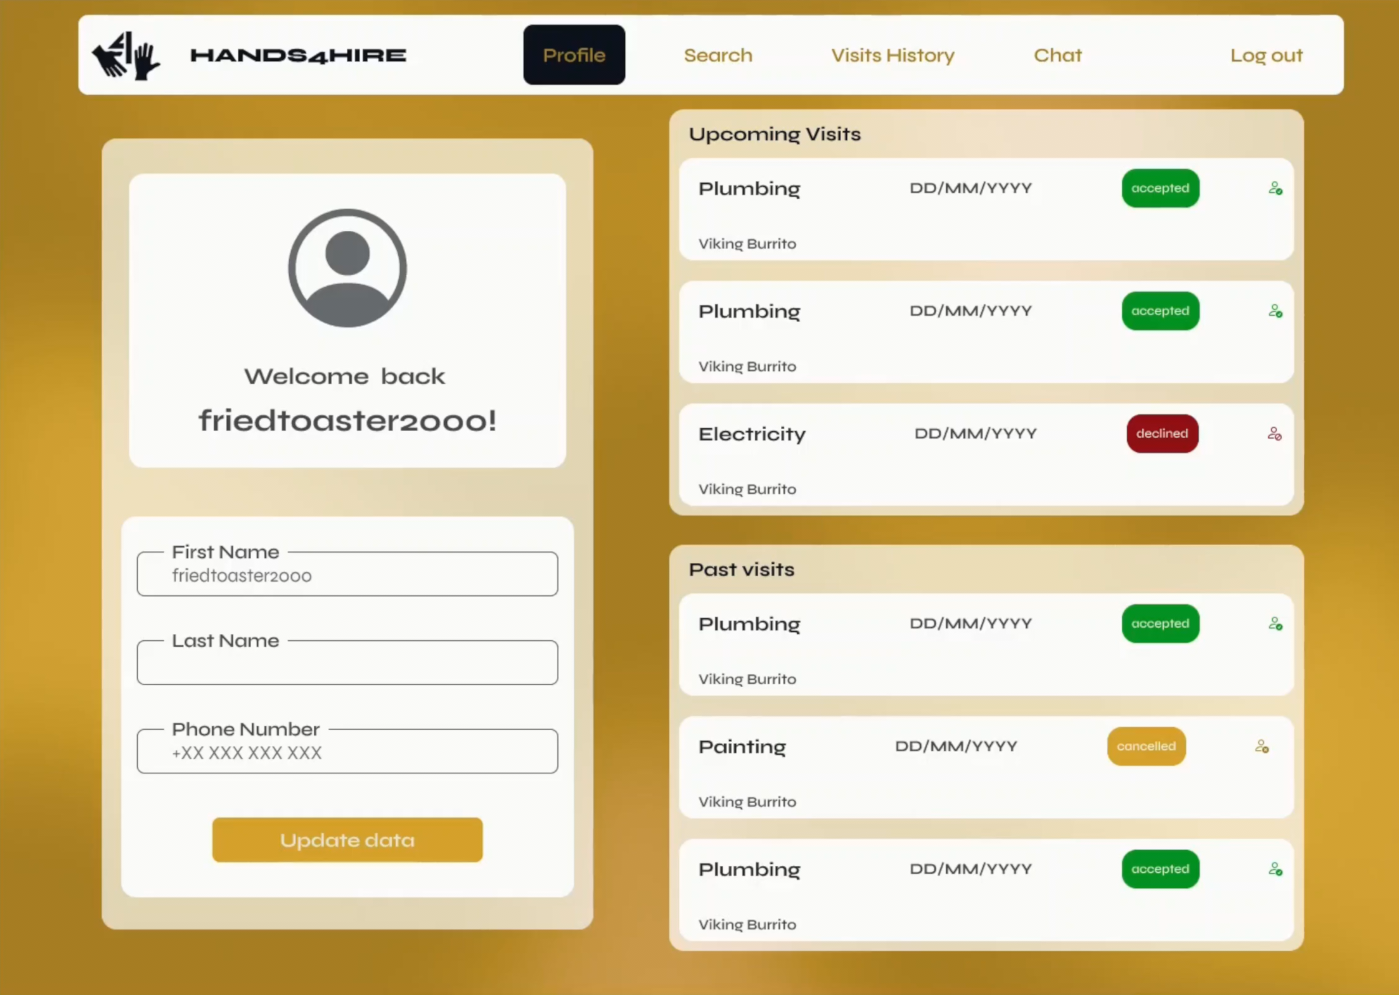
\includegraphics[width=\textwidth]{homepage_figma}
\caption{Homepage screen in Figma.}
\end{subfigure}%
\begin{subfigure}[t]{0.49\textwidth}
\centering
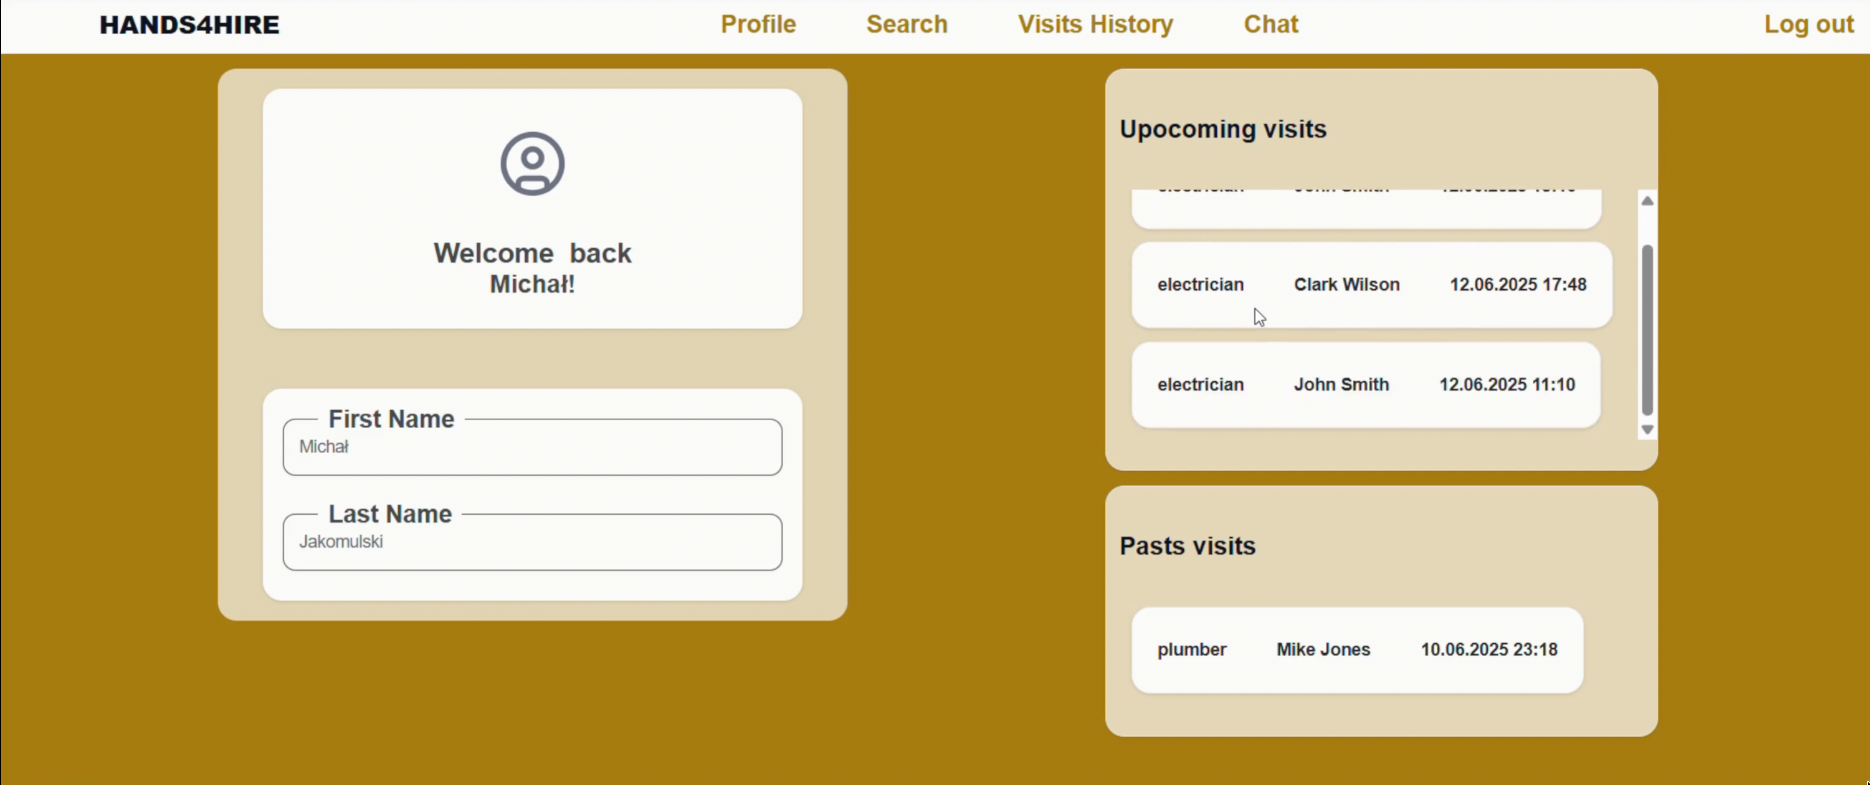
\includegraphics[width=\textwidth]{homepage_front}
\caption{Homepage screen in the App.}
\end{subfigure}%
\hfill
\begin{subfigure}[t]{0.49\textwidth}
\centering
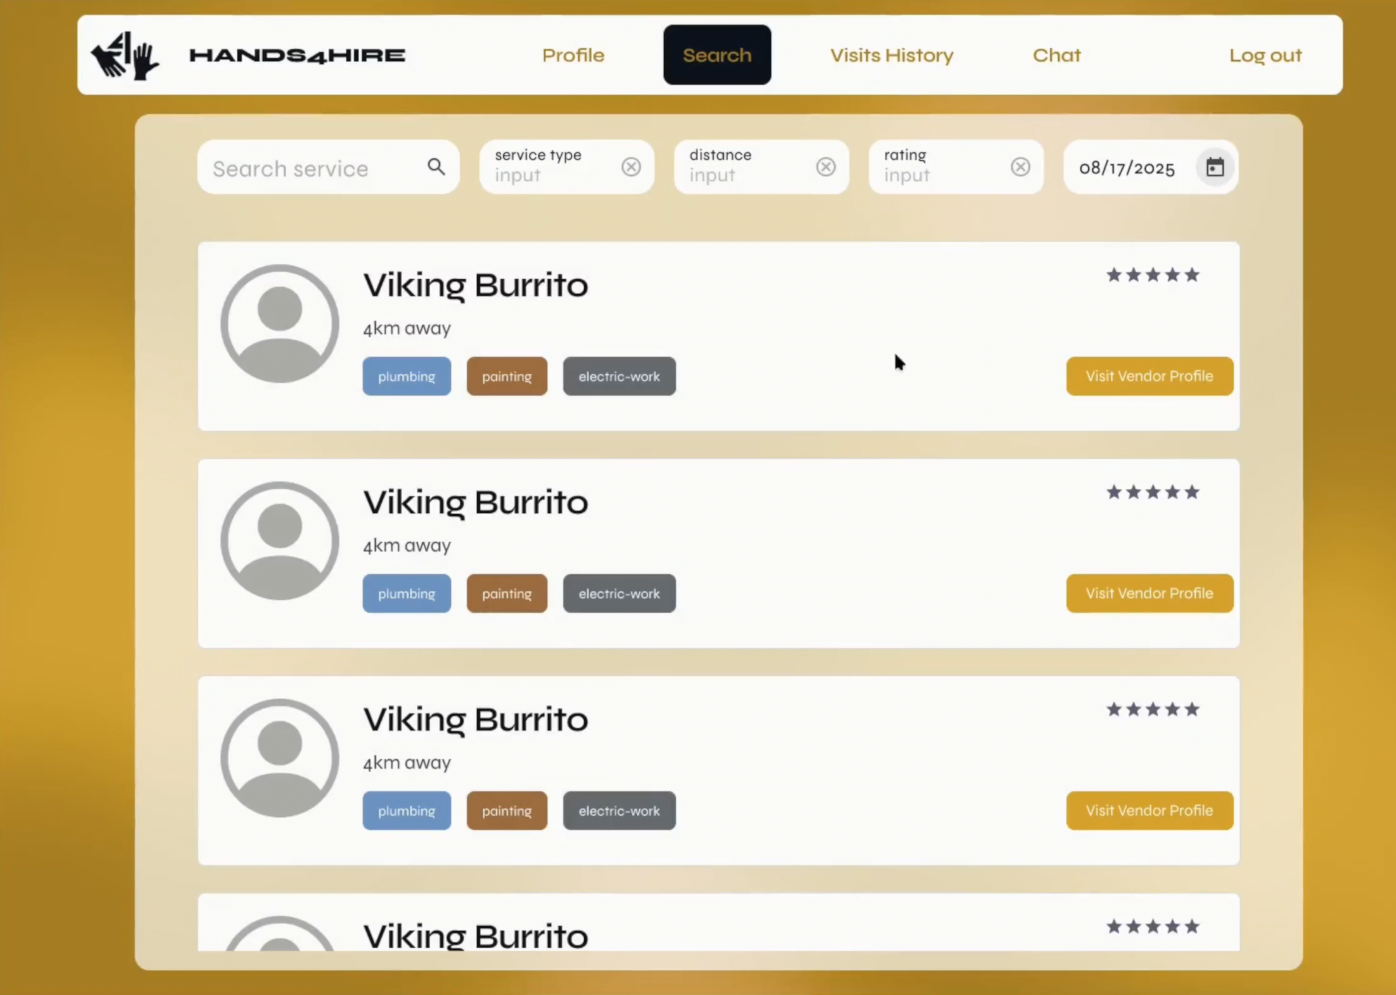
\includegraphics[width=\textwidth]{search_figma}
\caption{Vendor search screen in Figma.}
\end{subfigure}%
\begin{subfigure}[t]{0.49\textwidth}
\centering
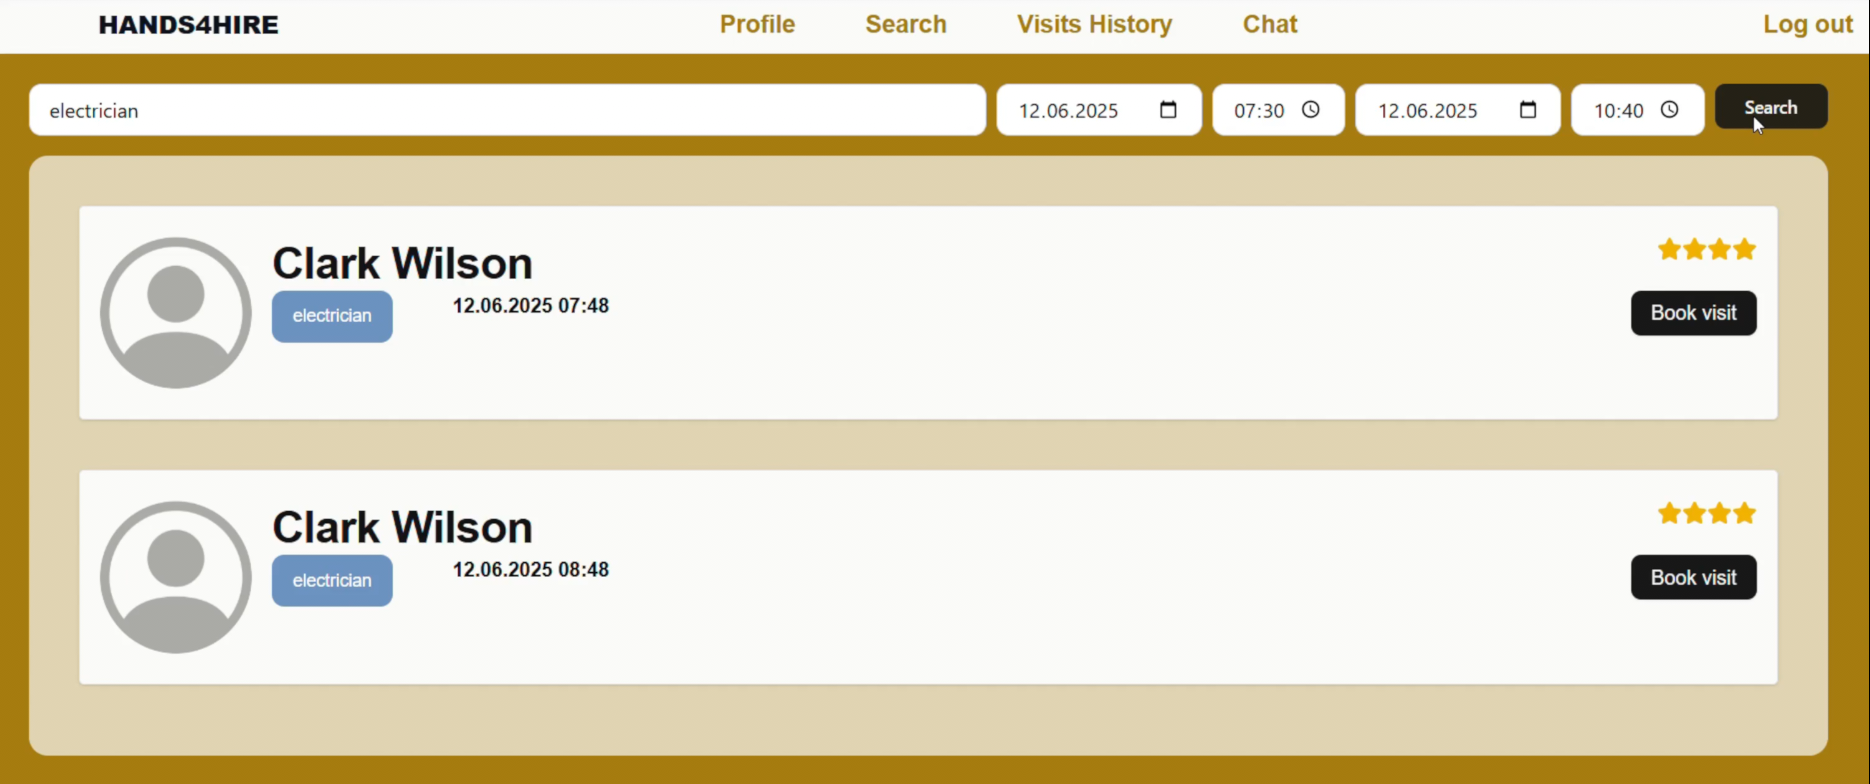
\includegraphics[width=\textwidth]{search_front}
\caption{Vendor search screen in the App.}
\end{subfigure}%

\caption[Frontend screens comparison.]{A side-by-side comparison of
Figma screens and Web Frontend pages.}
\label{fig:frontend_figma}
\end{figure}

\subsection{Kafka Service Communication}

Our platform primarily uses synchronous REST-based communication between microservices for direct operations. However, to decouple services, improve resilience, and handle asynchronous workflows in scenarios such as booking status change or user lifecycle status, we also integrate Apache Kafka as a messaging backbone.
Kafka was chosen due to its strong market position as a high-throughput, fault-tolerant event streaming platform. It integrates well with Google Cloud through Cloud Pub/Sub, making it a robust and scalable choice for inter-service communication within the ecosystem.
The design of our minimal integration is showcased in Figure \ref{fig:kafka-topics-diagram}.

\begin{figure}[H]
  \centering
  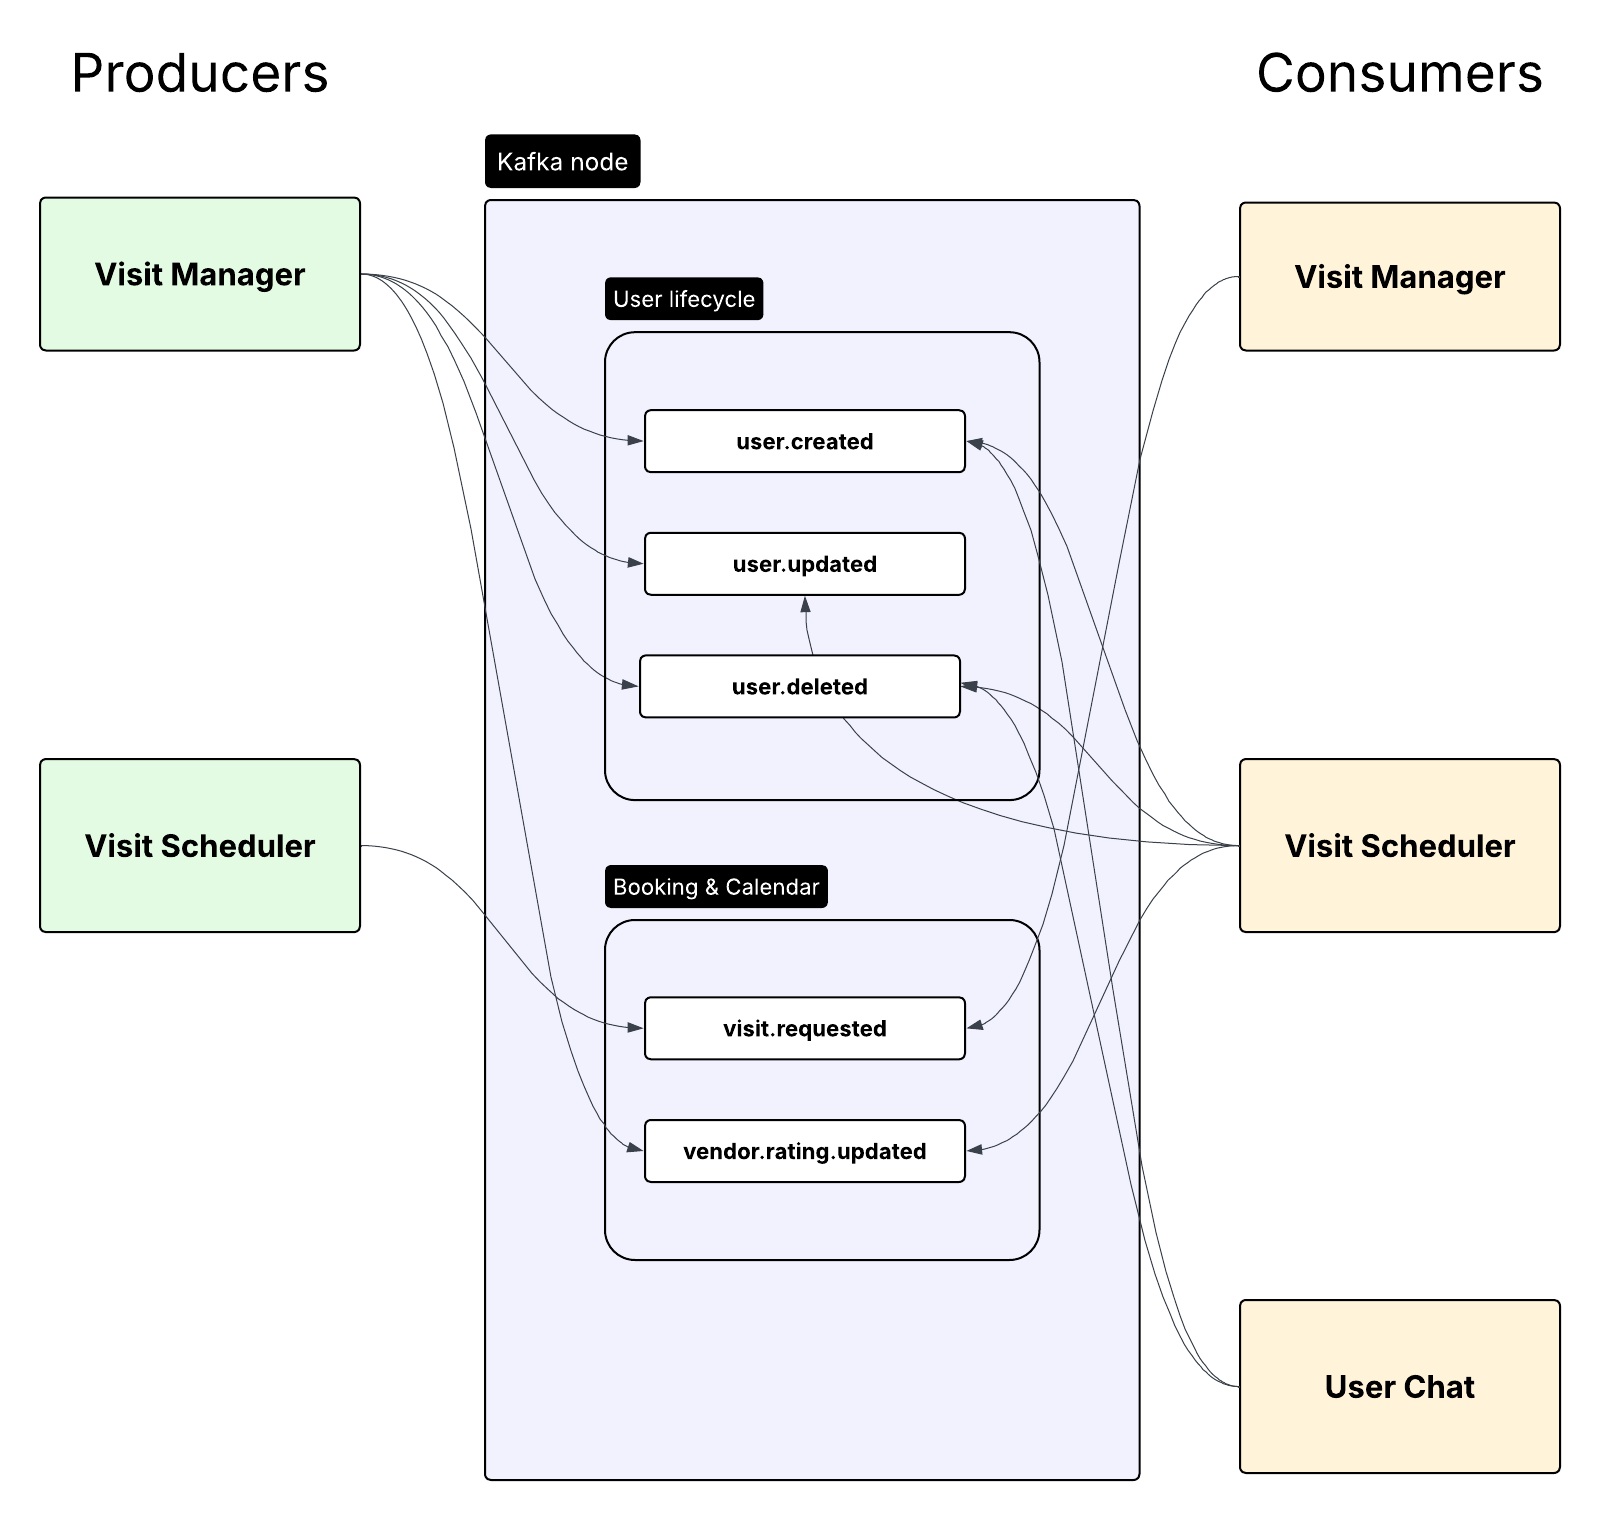
\includegraphics[width=\textwidth]{H4H_Kafka.png}
  \caption{Kafka Topics Diagram}
  \label{fig:kafka-topics-diagram}
\end{figure}

\subsection{Stripe integration}

The platform integrates Stripe for handling payment processing, specifically using the Stripe Payments simulation environment for development and testing. This integration allows us to model real-world transaction flows without incurring actual charges or needing production credentials during early development stages. We opted for the prebuilt Stripe Checkout solution, which offers a secure and PCI-compliant interface while reducing the need for custom implementation.

All payment-related interactions are handled through secure backend endpoints, which communicate with Stripe’s API over HTTPS. Webhooks are also configured in the simulated environment to test various payment outcomes (e.g., success, failure, cancellation). This setup enables the platform to fully validate and observe the payment lifecycle, ensuring a smooth transition to live payments in production when needed.

\subsection{Google OAuth2.0 Authentication}

For user authentication, the platform integrates Google OAuth 2.0, providing a secure, widely adopted login mechanism. It was chosen for its popularity, ease of use, and seamless integration with other Google Cloud services—ensuring a unified provider for both infrastructure and identity. By relying on Google’s ecosystem, we reduce complexity, avoid managing passwords directly, and benefit from built-in security features. 

\subsection{CI/CD Workflow \& Deployment}
\subsubsection{Source Control (GitHub)}
All code is version-controlled in GitHub. Each microservice resides
in a separate repository, with independent Dockerfiles and test configurations.
The project is available at \url{https://github.com/25l-ersms}.

\subsubsection{Development \& Production}

To streamline development and reduce cloud costs, our team worked primarily in a local development environment before deploying to production. This environment used \textbf{Docker Compose} for service orchestration—chosen over Minikube due to its lower overhead and better support for hot-reloading during rapid development.

To ensure code quality and consistency, the same rules applied both \textbf{pre-commit} (via hooks) and in CI pipelines, checking for formatting, linting, and test coverage. GitHub Actions automate this process, running on every push or merge to the main branch.

Reusable GitHub workflows were employed for tasks like pushing Docker images to Docker Hub, ensuring standardization across repositories. \textbf{Dependabot} was used for automated package dependency analysis, keeping images secure and up to date.

\begin{figure}
  \centering
  \fullpageimage{kubectl.png}
  \caption{Kubectl diagram}
  \label{fig:kubectl}
\end{figure}
Upon code push or merge to the main branch, when targeting the production environment, GitHub Actions executes
the following pipeline:
\begin{enumerate}
  \item \textbf{Build Docker Images}
  \item \textbf{Test}: Linting, unit tests, and integration tests are executed.
  \item \textbf{Push Docker Images} to Docker Hub.
  \item \textbf{Deploy to GKE} using kubectl and version-controlled
    Kubernetes manifests.
\end{enumerate}

Kubernetes manifests are defined and managed via Terraform, ensuring
infrastructure-as-code consistency and safe rollbacks.

\begin{figure}[H]
  \centering
  \fullpageimage{terraform.png}
  \caption{Terraform diagram}
  \label{fig:terraform}
\end{figure}

\section{Security \& Threat model}

\subsection{Implemented security measures}
\label{sub:security}

Security was a central consideration in the platform’s architecture, with decisions guided by a pragmatic threat model that prioritizes data integrity, access control, and system resilience. Several layers of defense were implemented across infrastructure, networking, and application layers.

\subsubsection{Backups and Replication}

To minimize data loss in case of infrastructure failure or misconfiguration, we propose a plan for daily backups taken for critical components: the entire GKE cluster, PostgreSQL, Firestore, and Elasticsearch. Both PostgreSQL and Firestore also benefit from Point-In-Time Recovery (PITR), allowing restoration of data up to seven days back. While, for simplicity reasons, compute resources are not replicated, all backups are replicated across zones, ensuring survivability even in the case of a full Google Cloud data center failure. Secrets, managed via GCP Secret Manager, are replicated by default.

\subsubsection{Secrets Management}

Sensitive credentials, such as API keys and database passwords, are never embedded in code. Instead, they are securely stored in GCP Secret Manager and synced into Kubernetes using the External Secrets Operator. This operator runs with its own IAM permissions and ensures that secrets are namespace-scoped and tightly controlled. This design enforces principle of least privilege across workloads.

\subsubsection{Network Security and Firewalls}

A defense-in-depth strategy was adopted with two firewall layers:
\begin{itemize}
\item \textbf{Cloudflare}, serving as a Web Application Firewall (WAF) and Content Delivery Network (CDN), handles edge-layer protection. It blocks DDoS attacks, enforces SSL/TLS encryption, and provides DNS, rate-limiting, and bot protection.
\item \textbf{GCP’s built-in} firewalls and \textbf{Application Load Balancer (ALB)} control internal traffic flow and route requests securely into the private GKE cluster.
\end{itemize}
    
Administrative access is further restricted via Identity-Aware Proxy (IAP) with IAM-based authentication, and in some cases, a socks proxy is used for access to the GKE cluster. Importantly, no inbound traffic is allowed directly—all requests must go through IAP or Cloudflare.

\subsubsection{Data Encryption}

All volumes—both ephemeral and persistent—are encrypted at rest, and this includes backups. Traffic in transit is also encrypted, whether it’s between services, to the load balancer, or to GCP-managed services (via Google’s Application Layer Transport Security, ALTS).

The security strategies outlined above were designed to address and mitigate a wide spectrum of potential risks, implemented as a direct response to the most critical threats identified during the platform's early threat modeling phase.

\subsection{STRIDE}

Threat modeling process has been conducted with accordance to the \textbf{STRIDE} framework.  
It was chosen for its structured way to analyze threats across various components of a system. Its broad coverage of both technical and procedural risks makes it particularly suitable for cloud-native, microservice-based architectures like ours. By applying STRIDE, we were able to identify vulnerabilities at both the infrastructure and application levels, ensuring that security concerns were proactively integrated into the design and implementation phases of the project.
Modeling process's outcome is showcased on the following pages as a single, summary document generated with the use of OWASP Threat Draagon modeling software. 

\begin{figure}[H]
  \centering
  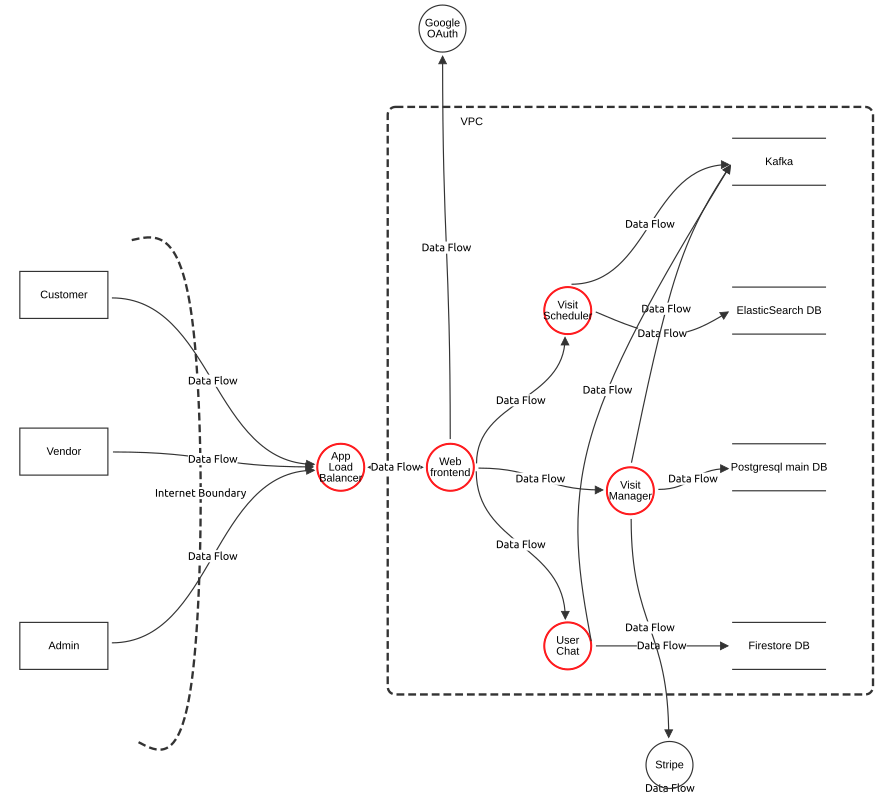
\includegraphics[width=\textwidth]{DFD-threat-model.png}
  \caption{Threat modeling Data Flow Diagram}
  \label{fig:DFD-threat-model}
\end{figure}


\includepdf[pages=-]{figures/H4H-threat-report.pdf}
\end{document}
